%% Copernicus Publications Manuscript Preparation Template for LaTeX Submissions
%% ---------------------------------
%% This template should be used for copernicus.cls
%% The class file and some style files are bundled in the Copernicus Latex Package, which can be downloaded from the different journal webpages.
%% For further assistance please contact Copernicus Publications at: production@copernicus.org
%% https://publications.copernicus.org/for_authors/manuscript_preparation.html


%% Please use the following documentclass and journal abbreviations for preprints and final revised papers.

%% 2-column papers and preprints
\documentclass[gmd, preprint]{copernicus}


%% Journal abbreviations (please use the same for preprints and final revised papers)


% Advances in Geosciences (adgeo)
% Advances in Radio Science (ars)
% Advances in Science and Research (asr)
% Advances in Statistical Climatology, Meteorology and Oceanography (ascmo)
% Aerosol Research (ar)
% Annales Geophysicae (angeo)
% Archives Animal Breeding (aab)
% Atmospheric Chemistry and Physics (acp)
% Atmospheric Measurement Techniques (amt)
% Biogeosciences (bg)
% Climate of the Past (cp)
% DEUQUA Special Publications (deuquasp)
% Earth Surface Dynamics (esurf)
% Earth System Dynamics (esd)
% Earth System Science Data (essd)
% E&G Quaternary Science Journal (egqsj)
% EGUsphere (egusphere) | This is only for EGUsphere preprints submitted without relation to an EGU journal.
% European Journal of Mineralogy (ejm)
% Fossil Record (fr)
% Geochronology (gchron)
% Geographica Helvetica (gh)
% Geoscience Communication (gc)
% Geoscientific Instrumentation, Methods and Data Systems (gi)
% Geoscientific Model Development (gmd)
% History of Geo- and Space Sciences (hgss)
% Hydrology and Earth System Sciences (hess)
% Journal of Bone and Joint Infection (jbji)
% Journal of Micropalaeontology (jm)
% Journal of Sensors and Sensor Systems (jsss)
% Magnetic Resonance (mr)
% Mechanical Sciences (ms)
% Natural Hazards and Earth System Sciences (nhess)
% Nonlinear Processes in Geophysics (npg)
% Ocean Science (os)
% Polarforschung - Journal of the German Society for Polar Research (polf)
% Primate Biology (pb)
% Proceedings of the International Association of Hydrological Sciences (piahs)
% Safety of Nuclear Waste Disposal (sand)
% Scientific Drilling (sd)
% SOIL (soil)
% Solid Earth (se)
% State of the Planet (sp)
% The Cryosphere (tc)
% Weather and Climate Dynamics (wcd)
% Web Ecology (we)
% Wind Energy Science (wes)


%% \usepackage commands included in the copernicus.cls:
%\usepackage[german, english]{babel}
\usepackage{tabularx}
%\usepackage{cancel}
%\usepackage{multirow}
%\usepackage{supertabular}
%\usepackage{algorithmic}
%\usepackage{algorithm}
%\usepackage{amsthm}
%\usepackage{float}
%\usepackage{subfig}
%\usepackage{rotating}
\usepackage[en-GB]{datetime2} % \usepackage[en-GB,en-US]{datetime2}
\DTMlangsetup[en-GB]{ord=raise,abbr,monthyearsep={,\space}}


%% define user commands
\newcommand{\mycomment}[1]{}

\begin{document}

\title{TEXT}


\title{Climate Forcing in Model Intercomparison Projects (MIPs): a review of evolution and future}
\mycomment{comment}

% \Author[affil]{given_name}{surname} % Author {first initial.}{last}
\Author[1]{Paul J.}{Durack} % ORCID 0000-0003-2835-1438
\Author[2]{the}{CMIP Forcing Task Team}
\Author[]{others please}{add yourselves}

% \affil % Affiliations
\affil[1]{Program for Climate Model Diagnosis and Intercomparison (PCMDI), Lawrence Livermore National Laboratory (LLNL), Livermore, California, USA}
\affil[2]{C/o CMIP International Project Office (CMIP-IPO), Harwell, UK}
\affil[]{Affiliation, location, country}

%% The [] brackets identify the author with the corresponding affiliation. 1, 2, 3, etc. should be inserted.

%% If an author is deceased, please mark the respective author name(s) with a dagger, e.g. "\Author[2,$\dag$]{Anton}{Smith}", and add a further "\affil[$\dag$]{deceased, 1 July 2019}".

%% If authors contributed equally, please mark the respective author names with an asterisk, e.g. "\Author[2,*]{Anton}{Smith}" and "\Author[3,*]{Bradley}{Miller}" and add a further affiliation: "\affil[*]{These authors contributed equally to this work.}".


\correspondence{Paul J. Durack (durack1@llnl.gov)}
\runningtitle{MIP forcing: Review and future}
\runningauthor{Durack et al.}


\received{}
\pubdiscuss{} %% only important for two-stage journals
\revised{}
\accepted{}
\published{}

%% These dates will be inserted by Copernicus Publications during the typesetting process.

\firstpage{1}
\maketitle


%% lift content from https://docs.google.com/document/d/1CF51lqguh-Zl9nZNJQu562ly780OI9Sa2tJciyCo5Zs/edit?skip_itp2_check=true&pli=1&tab=t.0 into this document



\begin{abstract}
Climate models are our most powerful tools for investigating global and regional climate changes caused by human and natural external forcing agents. These models are based on mathematical representations of the physics, chemistry, and biology of the climate system. Standardised experiments are constructed to quantify the climate model responses to externally imposed conditions, with these conditions often representing the observed past, or multiple hypothesized futures. These external imposed “forcing” conditions are captured in unique climate relevant agents, such as the natural influence of stratospheric sulphate aerosols from a large volcanic explosion, or human-driven components, such as enhancement to atmospheric carbon dioxide concentrations as a response to fossil fuel burning, or historical (or future) land use changes across the globe in response to changing human development.

The input4MIPs (input datasets for Model Intercomparison Projects) project was initiated to collect the forcing datasets produced for the 6th Phase of the Coupled Model Intercomparison Project (CMIP6; \citet{eyring_overview_2016}) available through the Earth System Grid Federation (ESGF; \citet{williams_global_2016}). The various datasets were collected to externally force climate models for the pre-industrial control (piControl), AMIP (Atmospheric Model Intercomparison Project), and historical experiments. Additional datasets are needed for many of the experiments that were performed as part of the CMIP6-endorsed community model intercomparison projects (MIPs; \citet{eyring_overview_2016}). Earlier versions of many of these datasets were used in the previous CMIP5 Project \citep{taylor_overview_2012} and before that in CMIP3 \citep{meehl_global_2007}, with far simpler configurations used in the preceding phases CMIP2 \citep{meehl_global_1995}), CMIP1 \citep{meehl_intercomparison_1997} and both AMIP2 and AMIP1 \citep{gleckler_amip_1999,gates_amip_1991}.

This paper describes the evolution of the CMIP6 project beyond that defined in \citet{eyring_overview_2016}. The project continued to grow as the phase was finalized, expanding from around 190 to 322 experiments at completion, with these experiments shared across a total of 23 community MIPs (Durack et al., 2025 [in prep]). 

{Compiled: \DTMnow}

\end{abstract}


\copyrightstatement{TEXT} %% This section is optional and can be used for copyright transfers.


\mycomment{Details about CMIP5 forcings can be found in https://pcmdi.llnl.gov/mips/cmip5/docs/Experiment_design_addendum.pdf}


\introduction  %% \introduction[modified heading if necessary]
Climate “forcings” are natural and anthropogenic (human-sourced) agents that influence the sign and magnitude of global and regional climate variability and change. For the CMIP6 historical experiment, the natural forcing agents include the observed incoming shortwave/solar radiation from the sun and the natural emission of sulphate aerosols from volcanic eruptions that have occurred throughout Earth’s history. For the CMIP6 historical experiment, anthropogenic forcing agents included the increasing atmospheric carbon dioxide concentrations (and other greenhouse gas species) that have been observed primarily due to fossil fuel burning, land use changes associated with human development, ozone, and nitrogen, short-lived climate forcers (SLCFs). In addition to externally imposed forcings, there are several natural forcings represented interactively in the models depending on their complexity. For example, emissions of biogenic volatile compounds, precursor for ozone and secondary aerosols, are typically simulated within models with full representation of atmospheric chemistry \citep{thornhill_climate-driven_2021,young_pre-industrial_2013}. These additional forcings...


\section{HEADING}
TEXT


% all figures and data should live in standalone github repo
\begin{figure}
    \centering
    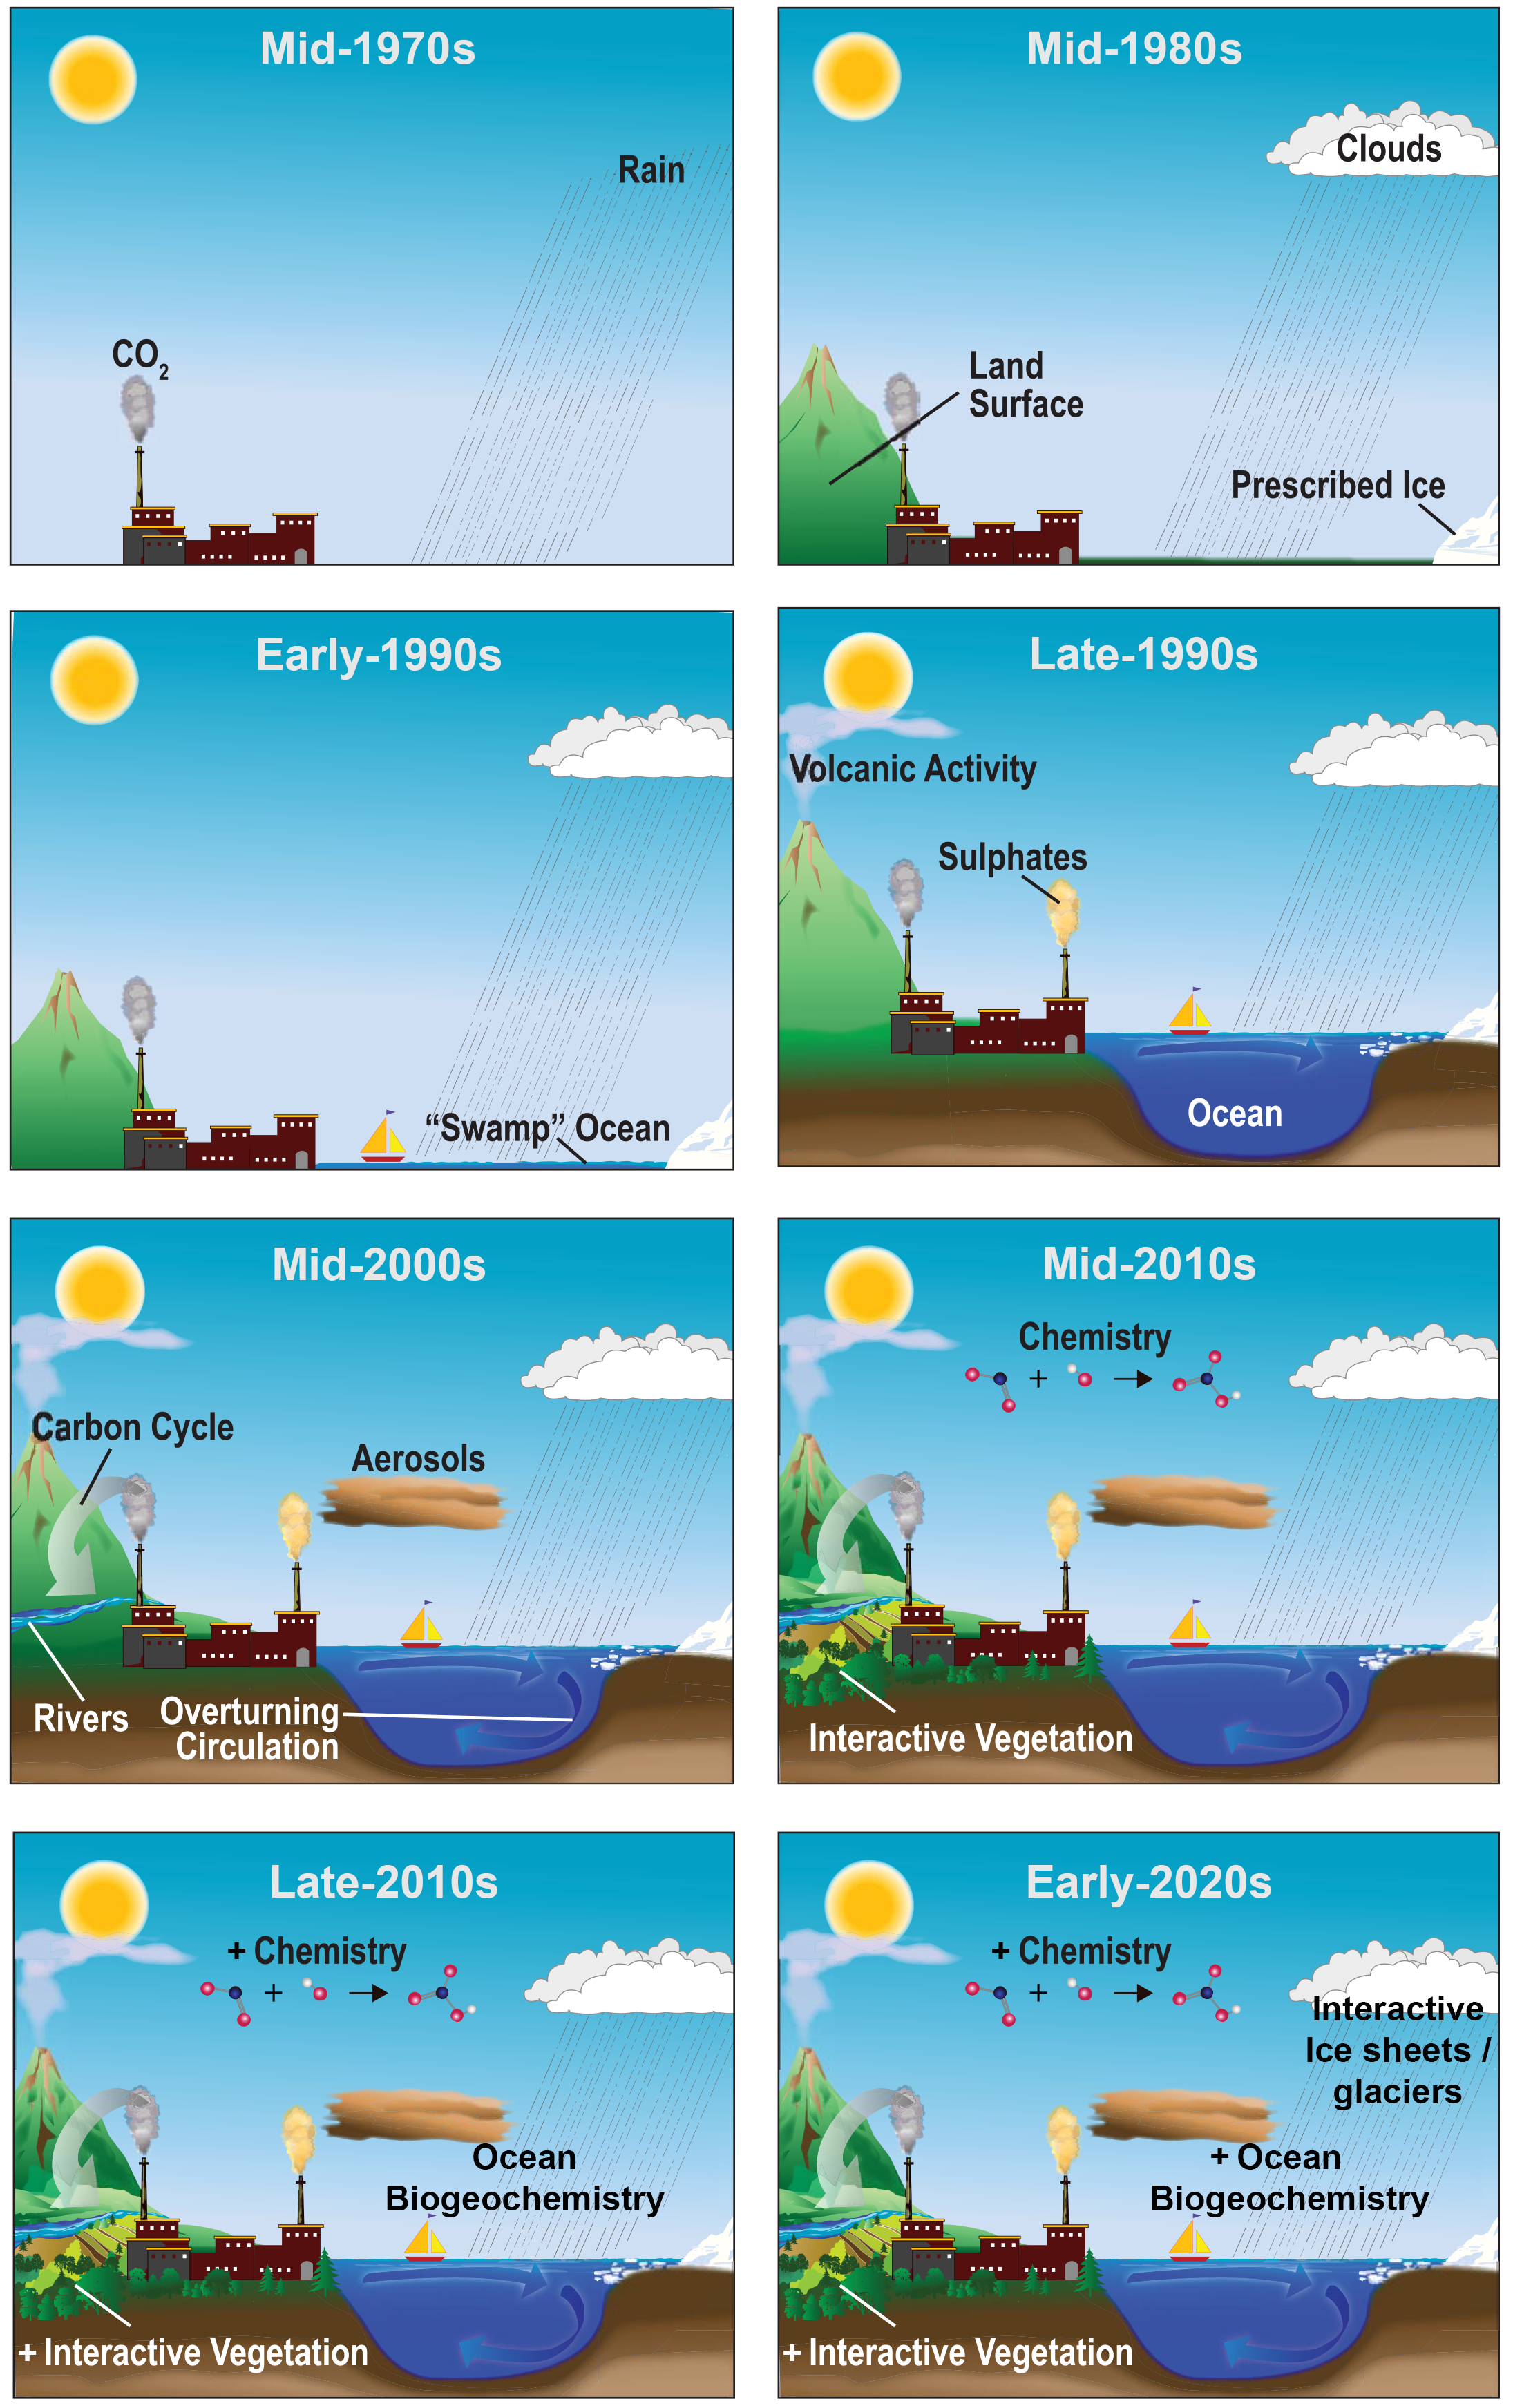
\includegraphics[width=1\linewidth]{AR4WG1_Ch01-p7-Fig1p2_adapted.png}
    \caption{Evolution of climate model complexity, the the early beginnings of atmosphere-only simulations (AGCM) in the 1970s, through more complex atmosphere-ocean coupled configurations (AOGCMs) in the late 1990s and early-to-mid 2000s, to Earth System Models (ESMs) in the 2010s onward. The increasing complexity approximates the evolution of climate model configurations, institutions, and countries contributing to completed Model Intercomparison Project (MIP) phases, from 1989 to today. As model complexity has increased, the number of external forcing agents required to best simulated our observed world and its changes have markedly increased}
    \label{fig:fig1-ModelComplexityThroughTime}
\end{figure}

% all figures and data should live in standalone github repo
\begin{figure}
    \centering
    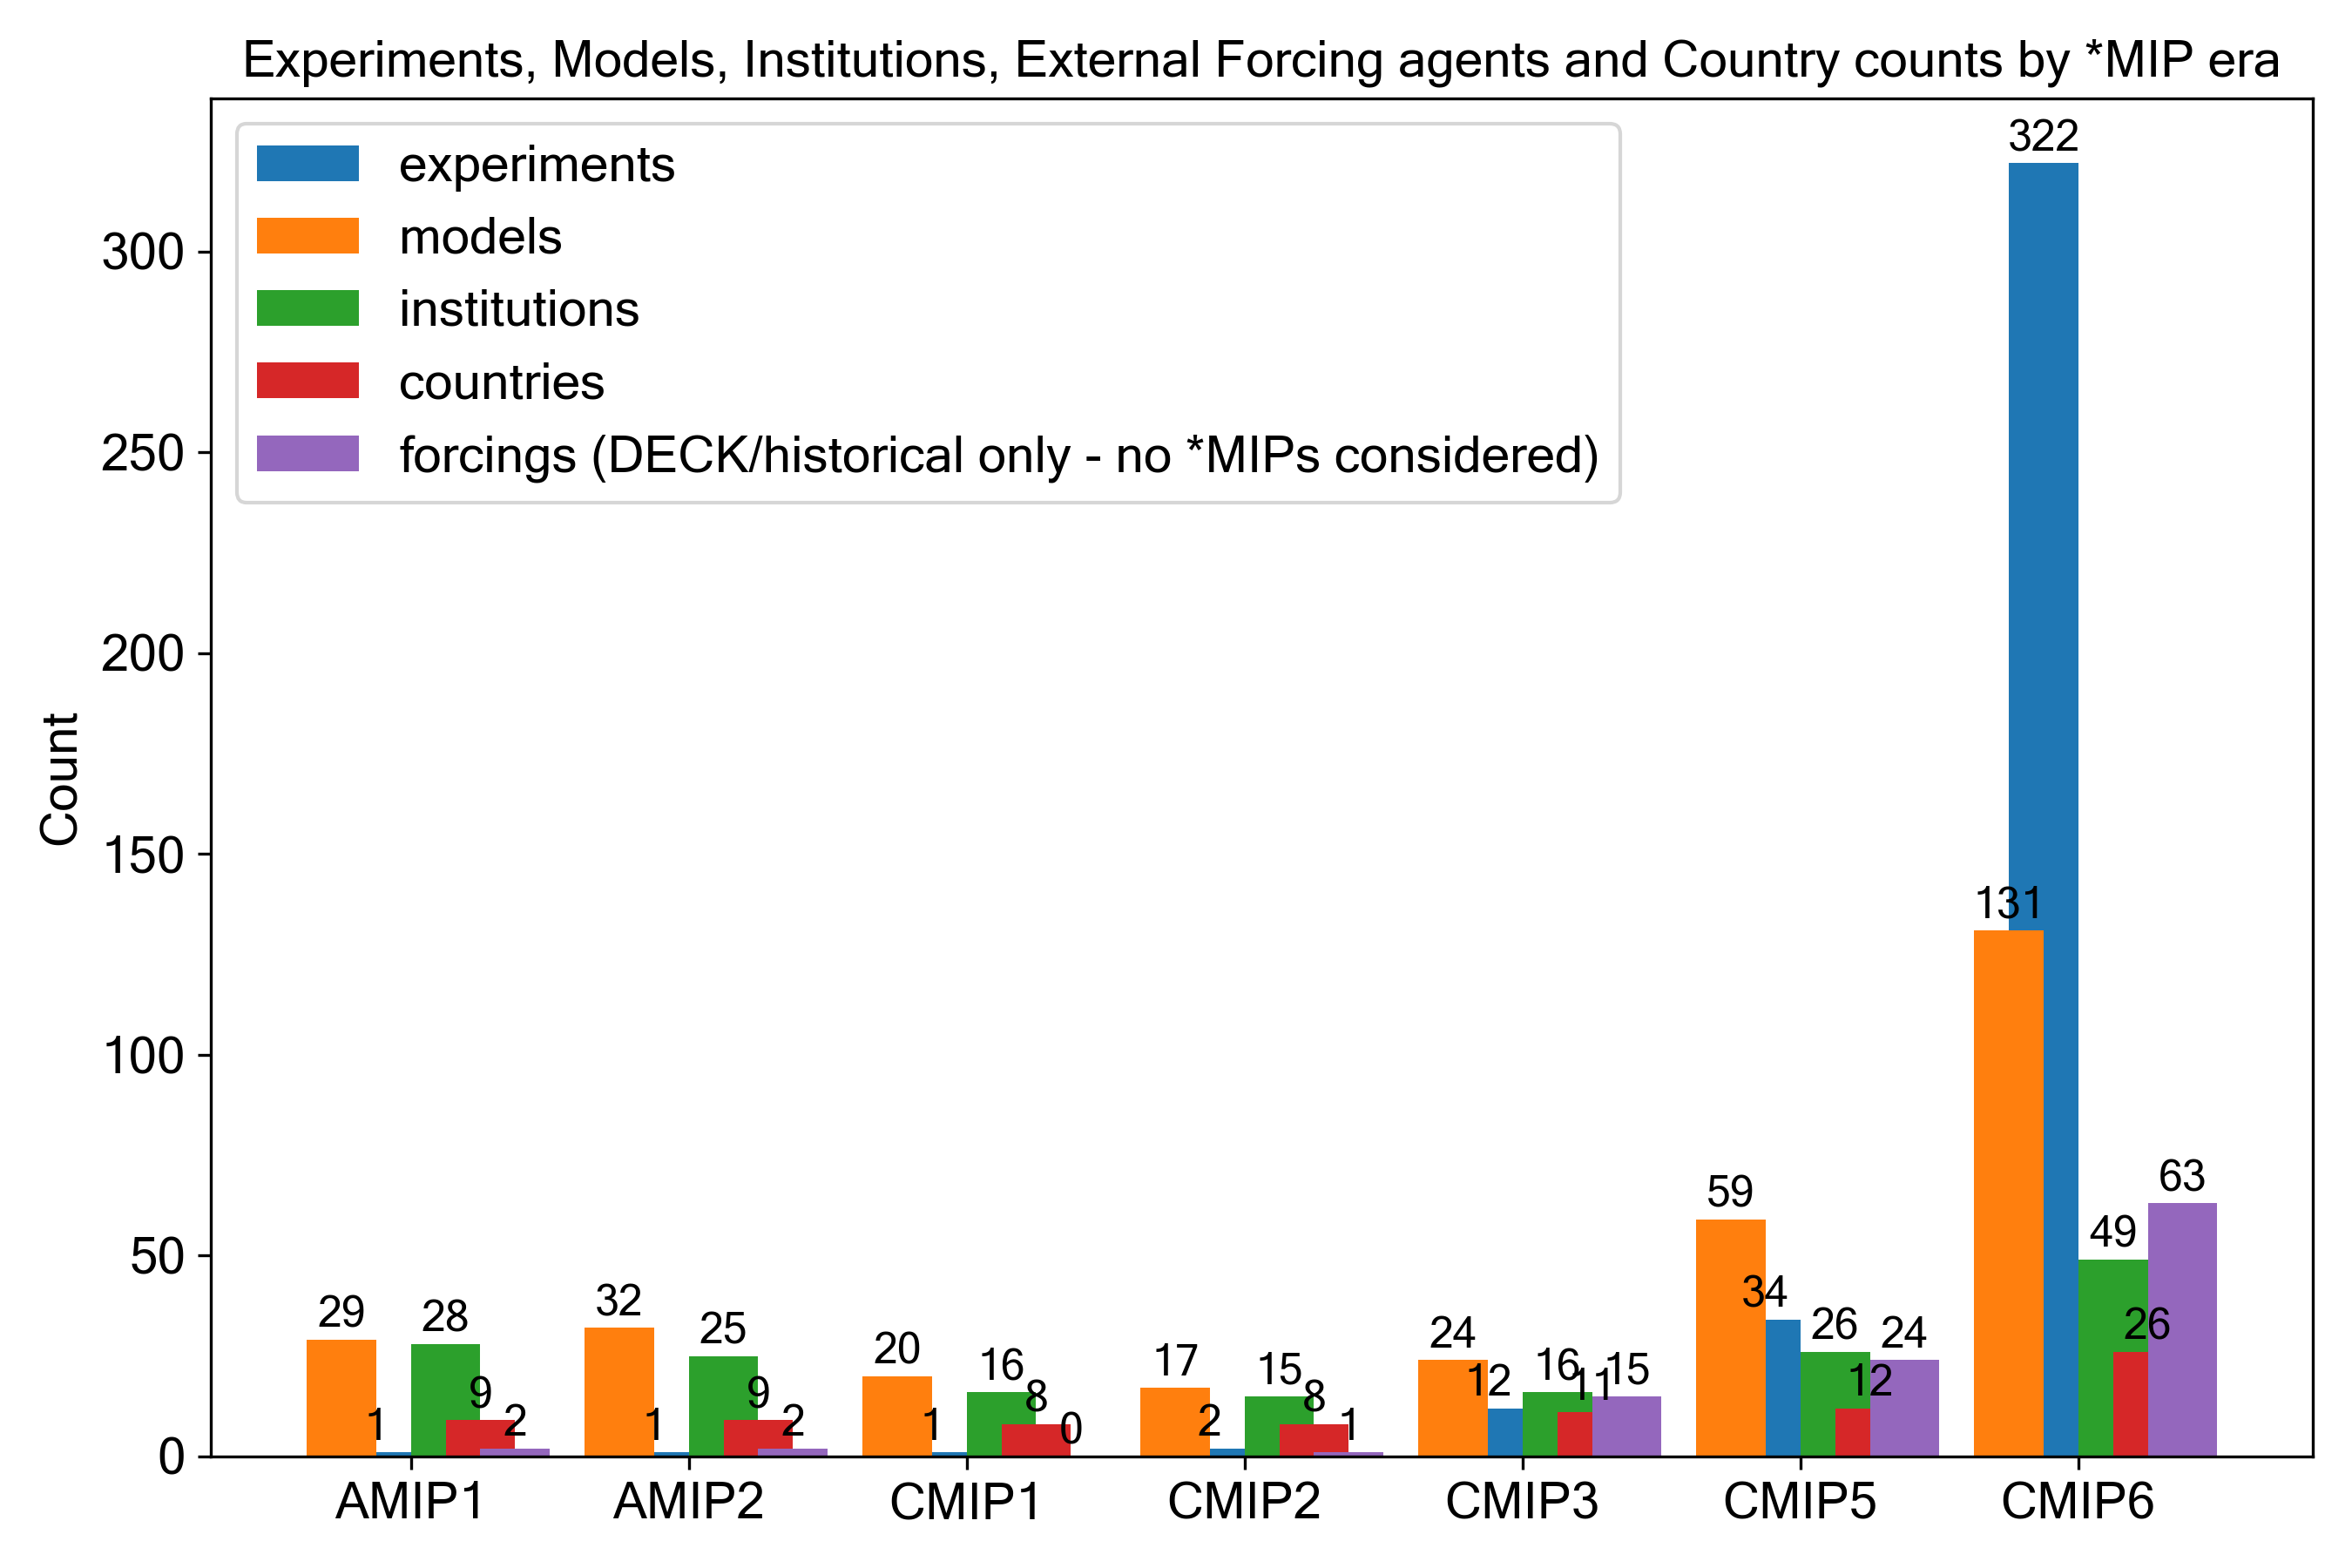
\includegraphics[width=1\linewidth]{230512T112843_MIPEvolution-Counts-plusForcing.png}
    \caption{Experiments, models, institutions, countries and forcing variants contributing to completed Model Intercomparison Project (MIP) phases, from 1989 to today (see \autoref{tab:tab1-ForcingByMIPsThroughTime}). The project's growth over the most recent phase reflects a growing community appetite for the latest climate data to inform decision-making, a distant evolution from the climate science origin of AMIP1. See Durack et al., 2025 [in prep] for an expansion of the experiment lists across MIP activities.}
    \label{fig:fig1-MIPGrowth}
\end{figure}


\begin{table*}[htp]
\renewcommand{\arraystretch}{1.5}
\scriptsize
\centering
\caption{Climate forcing across the Model Intercomparison Project (MIPs) phases, through time}
\resizebox{\textwidth}{!} {
\begin{tabularx}{0.9\textwidth} {
  | >{\raggedright\arraybackslash}X
  | >{\centering\arraybackslash}X
  | >{\centering\arraybackslash}X
  | >{\centering\arraybackslash}X
  | >{\centering\arraybackslash}X
  | >{\centering\arraybackslash}X
  | >{\centering\arraybackslash}X
  | >{\centering\arraybackslash}X
  | >{\centering\arraybackslash}X | }
\hline
\textbf{Forcing/MIP era} & \textbf{AMIP1} & \textbf{AMIP2} & \textbf{CMIP1} & \textbf{CMIP2} & \textbf{CMIP3} & \textbf{CMIP5} & \textbf{CMIP6} & \textbf{CMIP7}\\ \hline
\textbf{SSTs and sea ice (amip exp.)} & 1979-1988 & 1979-1996 & - & - & 1979-2002 & 1979-2008 & 1979-2014 & 1979-2021\\ \hline
\textbf{Greenhouse gases} & CO$_{2}$ 345 ppm (fixed) & CO$_{2}$ 345 ppm, CH$_{4}$ 1650 ppbv, N$_{2}$O 306 ppbv (fixed) & fixed & fixed and 1\% idealized & Y, 5 species & Y, 9 species & Y, 46 species & Y, 46 species\\ \hline
\textbf{Ozone} & - & climatology & - & fixed & Y, 1/2 groups & Y & Y & Y\\ \hline
\textbf{Sulphate aerosols (in/direct)} & - & climatology & - & - & Y, 1/2 groups & Y, 2/5 groups & Y & Y\\ \hline
\textbf{Black/organic carbon} & - & - & - & - & Y, 1/2 groups & Y, 4/5 groups & Y & Y\\ \hline
\textbf{Land use change} & - & active model component & - & - & Y, 1/3 groups & Y, 3/4 groups & 4 states & ?\\ \hline
\textbf{Solar irradiance} & 1365 Wm$^{-2}$ (fixed)& 1365 Wm$^{-2}$ (fixed) & fixed & fixed & Y, 1/2 groups & Y, 9/10 groups & Y & Y\\ \hline
\textbf{Volcanic aerosols} & - & - & - & - & Y, 1/2 groups & 3 variants, 9/10 groups & Y & Y\\ \hline
\textbf{Nitrogen deposition} & - & - & - & - & - & - & 4 species & ?\\ \hline
\textbf{Total varying forcings} & 2 & 2 & 0 & 1 (idealized) & $\sim$15 & $\sim$24 & $\sim$63 & ?\\ \hline
\textbf{Data delivery} & FTP & FTP & FTP, unspecified & FTP, unspecified & unspecified & unspecified & input4MIPs ESGF & input4MIPs ESGF\\ \hline
\end{tabularx}
} % /resizebox
\label{tab:tab1-ForcingByMIPsThroughTime}
\footnotesize{Note: estimates for CMIP3 and CMIP5 modelling group forcing data usage reproduced from \citet{santer_identification_2007}, and \citet{santer_human_2013} respectively}
\mycomment{
See slides - Durack/Fasullo https://docs.google.com/presentation/d/1_51Oohg4unT_W_F2xskYoOB3yIshMwxBBEnD6gIBI7Q/edit
Also see /Users/durack1/sync/Docs/admin/LLNL/24/240918_CERESScienceTeamMeeting-Oct24/241002a_durack1-CERESScienceTeamMeeting-ForcingsWhereWeveComeFromAndWhereWereGoing.pptx
}
\end{table*}


\subsection{HEADING}
TEXT


\subsubsection{HEADING}
TEXT


\conclusions  %% \conclusions[modified heading if necessary]
TEXT

%% The following commands are for the statements about the availability of data sets and/or software code corresponding to the manuscript.
%% It is strongly recommended to make use of these sections in case data sets and/or software code have been part of your research the article is based on.

\codeavailability{TEXT} %% use this section when having only software code available


\dataavailability{TEXT} %% use this section when having only data sets available


\codedataavailability{TEXT} %% use this section when having data sets and software code available


\sampleavailability{TEXT} %% use this section when having geoscientific samples available


\videosupplement{TEXT} %% use this section when having video supplements available


\appendix
\section{}    %% Appendix A

\subsection{}     %% Appendix A1, A2, etc.


\noappendix       %% use this to mark the end of the appendix section. Otherwise the figures might be numbered incorrectly (e.g. 10 instead of 1).

%% Regarding figures and tables in appendices, the following two options are possible depending on your general handling of figures and tables in the manuscript environment:

%% Option 1: If you sorted all figures and tables into the sections of the text, please also sort the appendix figures and appendix tables into the respective appendix sections.
%% They will be correctly named automatically.

%% Option 2: If you put all figures after the reference list, please insert appendix tables and figures after the normal tables and figures.
%% To rename them correctly to A1, A2, etc., please add the following commands in front of them:

\appendixfigures  %% needs to be added in front of appendix figures

\appendixtables   %% needs to be added in front of appendix tables

%% Please add \clearpage between each table and/or figure. Further guidelines on figures and tables can be found below.



\authorcontribution{TEXT} %% this section is mandatory

\competinginterests{TEXT} %% this section is mandatory even if you declare that no competing interests are present

\disclaimer{TEXT} %% optional section

\begin{acknowledgements}
TEXT
\end{acknowledgements}




%% REFERENCES

%% The reference list is compiled as follows:
%\begin{thebibliography}{}
%\bibitem[AUTHOR(YEAR)]{LABEL1}
%REFERENCE 1
%\bibitem[AUTHOR(YEAR)]{LABEL2}
%REFERENCE 2
%\end{thebibliography}
\bibliographystyle{copernicus}
\bibliography{241114a}


%% Since the Copernicus LaTeX package includes the BibTeX style file copernicus.bst,
%% authors experienced with BibTeX only have to include the following two lines:
%%
%% \bibliographystyle{copernicus}
%% \bibliography{example.bib}
%%
%% URLs and DOIs can be entered in your BibTeX file as:
%%
%% URL = {http://www.xyz.org/~jones/idx_g.htm}
%% DOI = {10.5194/xyz}


%% LITERATURE CITATIONS
%%
%% command                        & example result
%% \citet{jones90}|               & Jones et al. (1990)
%% \citep{jones90}|               & (Jones et al., 1990)
%% \citep{jones90,jones93}|       & (Jones et al., 1990, 1993)
%% \citep[p.~32]{jones90}|        & (Jones et al., 1990, p.~32)
%% \citep[e.g.,][]{jones90}|      & (e.g., Jones et al., 1990)
%% \citep[e.g.,][p.~32]{jones90}| & (e.g., Jones et al., 1990, p.~32)
%% \citeauthor{jones90}|          & Jones et al.
%% \citeyear{jones90}|            & 1990



%% FIGURES

%% When figures and tables are placed at the end of the MS (article in one-column style), please add \clearpage
%% between bibliography and first table and/or figure as well as between each table and/or figure.

% The figure files should be labelled correctly with Arabic numerals (e.g. fig01.jpg, fig02.png).


%% ONE-COLUMN FIGURES

%%f
%\begin{figure}[t]
%\includegraphics[width=8.3cm]{FILE NAME}
%\caption{TEXT}
%\end{figure}
%
%%% TWO-COLUMN FIGURES
%
%%f
%\begin{figure*}[t]
%\includegraphics[width=12cm]{FILE NAME}
%\caption{TEXT}
%\end{figure*}
%
%
%%% TABLES
%%%
%%% The different columns must be seperated with a & command and should
%%% end with \\ to identify the column brake.
%
%%% ONE-COLUMN TABLE
%
%%t
%\begin{table}[t]
%\caption{TEXT}
%\begin{tabular}{column = lcr}
%\tophline
%
%\middlehline
%
%\bottomhline
%\end{tabular}
%\belowtable{} % Table Footnotes
%\end{table}
%
%%% TWO-COLUMN TABLE
%
%%t
%\begin{table*}[t]
%\caption{TEXT}
%\begin{tabular}{column = lcr}
%\tophline
%
%\middlehline
%
%\bottomhline
%\end{tabular}
%\belowtable{} % Table Footnotes
%\end{table*}
%
%%% LANDSCAPE TABLE
%
%%t
%\begin{sidewaystable*}[t]
%\caption{TEXT}
%\begin{tabular}{column = lcr}
%\tophline
%
%\middlehline
%
%\bottomhline
%\end{tabular}
%\belowtable{} % Table Footnotes
%\end{sidewaystable*}
%
%
%%% MATHEMATICAL EXPRESSIONS
%
%%% All papers typeset by Copernicus Publications follow the math typesetting regulations
%%% given by the IUPAC Green Book (IUPAC: Quantities, Units and Symbols in Physical Chemistry,
%%% 2nd Edn., Blackwell Science, available at: http://old.iupac.org/publications/books/gbook/green_book_2ed.pdf, 1993).
%%%
%%% Physical quantities/variables are typeset in italic font (t for time, T for Temperature)
%%% Indices which are not defined are typeset in italic font (x, y, z, a, b, c)
%%% Items/objects which are defined are typeset in roman font (Car A, Car B)
%%% Descriptions/specifications which are defined by itself are typeset in roman font (abs, rel, ref, tot, net, ice)
%%% Abbreviations from 2 letters are typeset in roman font (RH, LAI)
%%% Vectors are identified in bold italic font using \vec{x}
%%% Matrices are identified in bold roman font
%%% Multiplication signs are typeset using the LaTeX commands \times (for vector products, grids, and exponential notations) or \cdot
%%% The character * should not be applied as mutliplication sign
%
%
%%% EQUATIONS
%
%%% Single-row equation
%
%\begin{equation}
%
%\end{equation}
%
%%% Multiline equation
%
%\begin{align}
%& 3 + 5 = 8\\
%& 3 + 5 = 8\\
%& 3 + 5 = 8
%\end{align}
%
%
%%% MATRICES
%
%\begin{matrix}
%x & y & z\\
%x & y & z\\
%x & y & z\\
%\end{matrix}
%
%
%%% ALGORITHM
%
%\begin{algorithm}
%\caption{...}
%\label{a1}
%\begin{algorithmic}
%...
%\end{algorithmic}
%\end{algorithm}
%
%
%%% CHEMICAL FORMULAS AND REACTIONS
%
%%% For formulas embedded in the text, please use \chem{}
%
%%% The reaction environment creates labels including the letter R, i.e. (R1), (R2), etc.
%
%\begin{reaction}
%%% \rightarrow should be used for normal (one-way) chemical reactions
%%% \rightleftharpoons should be used for equilibria
%%% \leftrightarrow should be used for resonance structures
%\end{reaction}
%
%
%%% PHYSICAL UNITS
%%%
%%% Please use \unit{} and apply the exponential notation


\end{document}
